\documentclass[
  tikz, convert={density=800, size=2600x1300, outext=.png}, 
  background, border=0.5cm
 ]{standalone}
\usepackage{amsmath, amssymb, amsthm, bm, bbm, xcolor}

\usetikzlibrary{shapes.geometric, positioning}
\usetikzlibrary{quotes, angles, calc, backgrounds}
\definecolor{BadgerRed}{cmyk}{0.03, 1, 0.66, 0.12}

\definecolor{myColor1}{RGB}{153,153,153}
\definecolor{myColor2}{RGB}{230,159,0}
\definecolor{myColor3}{RGB}{86,180,233}
\definecolor{myColor4}{RGB}{0,158,115}
\definecolor{myColor5}{RGB}{240,228,66}
\definecolor{myColor6}{RGB}{0,114,178}
\definecolor{myColor7}{RGB}{213,94,0}
\definecolor{myColor8}{RGB}{204,121,167}

\tikzset{decisionNode/.style={inner sep=5pt, shape=circle,align=center,font=\Large,draw, fill=gray!40}}
\tikzset{leafNode/.style={inner sep=5pt, shape=circle, align=center, font = \Large, draw, fill=white}}
\tikzset{decisionRule/.style={shape=rectangle, align=center, font = \normalsize, draw=none, fill=white}}
\tikzset{jump/.style={shape=rectangle, align=center, font=\Large, draw=none, fill=white}}
\tikzset{annotation/.style={shape=rectangle, align=center, font=\Large, draw=none, fill=white}}

\begin{document}



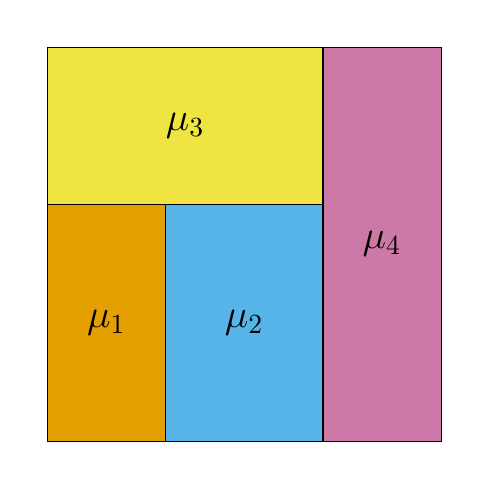
\begin{tikzpicture}[scale=5,
  background rectangle/.style={fill=white}, show background rectangle,
  level 1/.style={sibling distance = 9em},
  level 2/.style={sibling distance = 6em},
  level 3/.style={sibling distance = 3em},
  level 4/.style={sibling distance = 4em},
  level distance = 4em]
  
\useasboundingbox (-0.05, -0.05) rectangle (1.05, 1.05);

\draw (0,0) rectangle (1,1);
\draw[fill = myColor8] (0.7,0) rectangle (1,1) node[pos = 0.5]{\Large $\mu_{4}$};
\draw[fill = myColor5] (0,0.6) rectangle (0.7,1) node[pos = 0.5]{\Large $\mu_{3}$};
\draw[fill = myColor3] (0.3,0) rectangle (0.7, 0.6) node[pos = 0.5]{\Large $\mu_{2}$};
\draw[fill = myColor2] (0,0) rectangle (0.3, 0.6) node[pos = 0.5] {\Large $\mu_{1}$};
  
\end{tikzpicture}
\end{document}